\section{\gls{ims} dataset No.1 - Bearing 3x sensor}
\label{sec:ValidationOnRealWorldData}
\begin{figure}
    \centering
    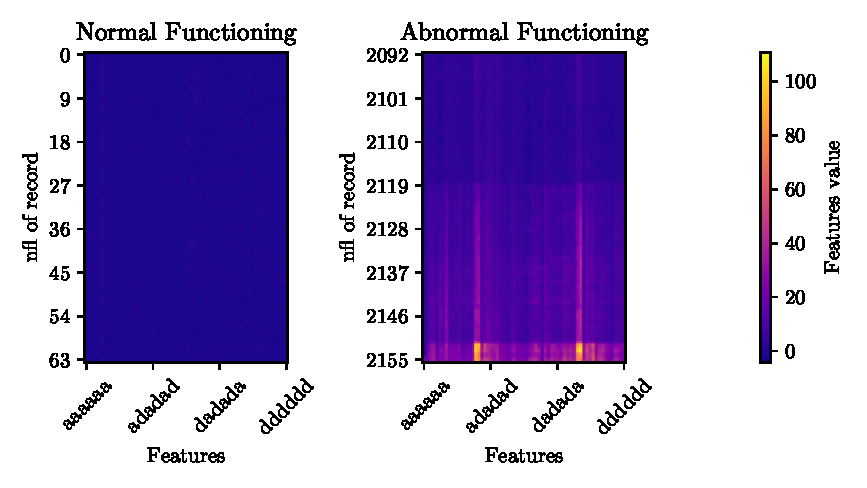
\includegraphics{images/IMS/Heatmap.pdf}
    \caption{Heatmap of the \gls{glo:std} \gls{glo:feature}s value for the test $\text{n}^\circ$1 of \gls{ims} dataset}
    \label{fig:Heatmap}
\end{figure}


To start the validation, the test No.1 of the \gls{ims} dataset is subdivided into \emph{training} and \emph{testing} datasets. The first 500 samples are used for training, and the remaining samples are used for testing. 

For all the algorithms, the assumption about the system is that, even if the degradation is continuous, the system is surely healthy until 2003-11-07. The threshold for performing the \gls{nd} is set conformingly to this assumption, for every model considered. Otherwise, the performance of any model could be artificially made as good as desired, by simply setting the threshold to a lower value.

The configuration file is set to use the data from the \quoted{bearing 3x} sensor, extracting all the time-domain and frequency-domain \gls{glo:feature}s described in \autoref{ch:FeatureExtraction}. The training dataset is used to train the \gls{mla} to recognize the normal behaviour of the bearing, and the testing dataset is used to validate the trained model. The \autoref{tab:IMS_test_parameters} shows the parameters of test No.1 of the \gls{ims} dataset. For display purposes, the \gls{glo:feature}s are \gls{glo:std}, and the heatmap of the \gls{glo:std} \gls{glo:feature}s is shown in \autoref{fig:Heatmap} in normal and abnormal conditions.

The abstract version of the \gls{fieldAg} has been used to extract the \gls{glo:feature}s from the dataset, creating all the \gls{glo:snap}s in the set $\gls{sym:snapset}=\{\gls{sym:snap}_1,\gls{sym:snap}_2,\dots,\gls{sym:snap}_{500}\}$. These \gls{glo:snap}s are stored in the \emph{unconsumed} collection of the database.

\subsection{Training - K-means}

Using the commands of the \gls{cli}, the training procedure has been launched:
\begin{minted}[linenos,breaklines]{bash}
    C:/Users/JohnSmith/Code/framework> python ./MASTER.py run-\gls{glo:feature}-\gls{glo:agent}
    C:/Users/JohnSmith/Code/framework> python ./MASTER.py run-machine-learning-\gls{glo:agent} novelty train
\end{minted}

where the first command runs the \gls{fieldAg} and the second one runs an \quoted{healthy} instance of the \gls{mla} in training mode.
At this point, the \gls{mla} asks the user to move the \gls{glo:snap}s from the \emph{unconsumed} to the \emph{healthy} collection, since the \emph{healthy} collection is empty. After the confirmation, the \gls{mla} starts the training with a different number of \gls{glo:clust}s and outputs the scoring in the form of silhouette and inertia scores. The results are shown in \autoref{fig:SilScore_01} and \autoref{fig:InertiaScore_01}. The user can confirm that the best number of \gls{glo:clust}s is 2, as the silhouette score is the highest and the inertia score is at the \gls{pof} point, or insert another number of \gls{glo:clust}s, remembering that it is best to overestimate the number of \gls{glo:clust}s to increase the system sensitivity, as discussed in \autoref{sec:wrong_k}. 

In this case, the number of \gls{glo:clust}s has been set to 2, so that the \gls{mla} saves the model trained with $n=2$ into the database. Even if the \gls{glo:feature} space has high dimensionality, the \gls{glo:agent} plot to the user also a scatter plot of a subset of \gls{glo:feature}s of the training dataset, to have a visual feedback of the \gls{glo:clust}ing, as shown in \autoref{fig:Clusters}, where the points are the \gls{glo:snap}s, the crosses are the centroids and the colours represent the assigned \gls{glo:clust}. We can observe that selecting 2 as the number of \gls{glo:clust}s is adequate and that the projections of the \gls{glo:clust}s' shapes on some planes are not perfectly spherical but, at least, they are not too elongated. This is a good sign for the K-means algorithm, as discussed in \autoref{sec:kmeans_limits}.

\begin{figure}
    \centering
    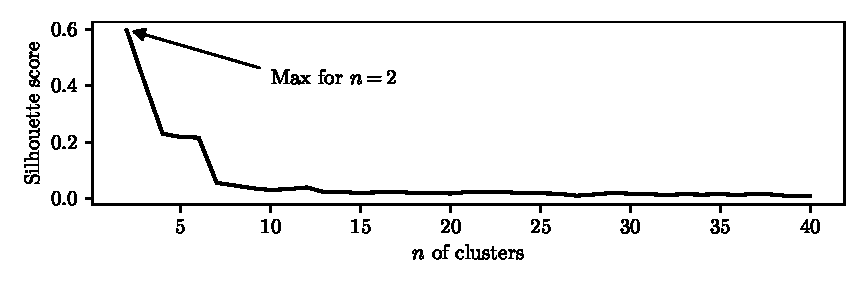
\includegraphics{images/IMS/SilScore_01.pdf}
    \caption{Silhouette score for \gls{glo:clust}ing the test $\text{n}^\circ$1 of \gls{ims} dataset (K-means)}
    \label{fig:SilScore_01}
\end{figure}

\begin{figure}
    \centering
    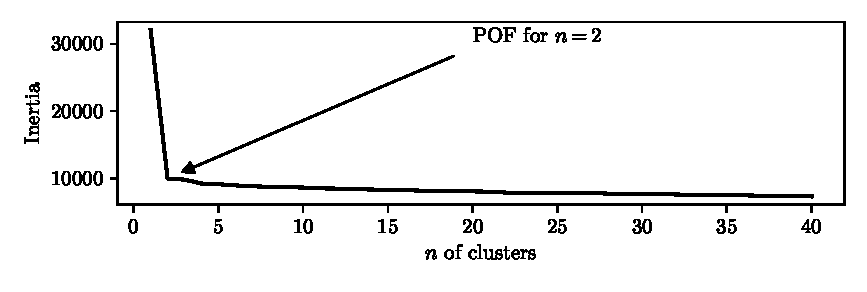
\includegraphics{images/IMS/InertiaScore_01.pdf}
    \caption{Inertia score for \gls{glo:clust}ing the test $\text{n}^\circ$1 of \gls{ims} dataset (K-means)}
    \label{fig:InertiaScore_01}
\end{figure}

\begin{figure}
    \centering
    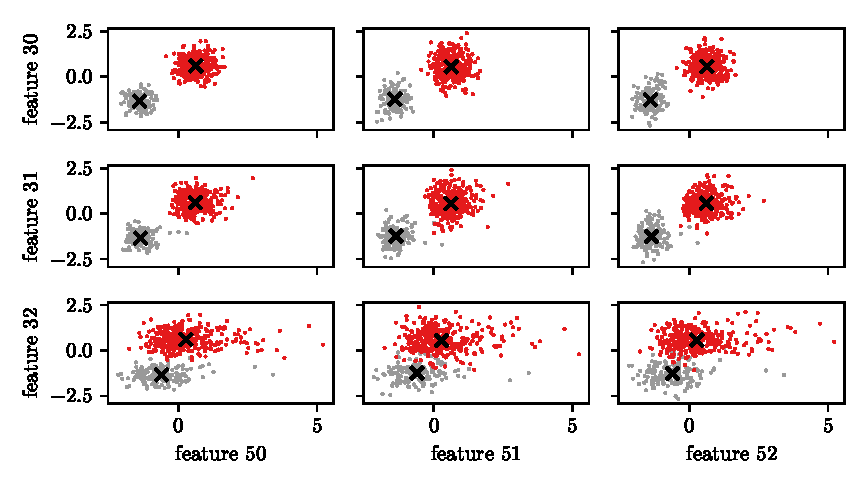
\includegraphics{images/IMS/Clusters.pdf}
    \caption{Scatterplot of training $\gls{glo:snap}$ for the test $\text{n}^\circ$1 of \gls{ims} dataset}
    \label{fig:Clusters}
\end{figure}

\subsection{\gls{nd} Validation - K-means}
Using the validation partition of the dataset, it is possible to set the \gls{mla} in \emph{evaluate} mode. The \gls{fieldAg} uses the validation partition and fills the \emph{raw} collection with the time-series. The {\gls{fa}} extract the \gls{glo:feature}s and continuously fill the \emph{unconsumed} collection with the \gls{glo:snap}s. The \gls{mla} evaluates the \gls{glo:snap}s according to \autoref{alg:eval_new_snapshot}  and plots the result, as well as generating a warning if the novelty metric is greater than a certain threshold (in this case 50\%, but it is configurable in the usual \texttt{.yaml} file). The results are shown in \autoref{fig:NoveltyScore_01}, where we can see that the \gls{glo:frmwrk} detects the novelty quite early, at 2003-11-16 07:46, while the dataset authors, declared the test finished because of bearing defects (not catastrophic failures) at 2003-11-25 23:40. The comparison of the margin of early detection for different algorithms will be resumed later.

In \autoref{fig:NoveltyScore_01_detail}, a detailed view of the \gls{nd} metric becoming consistently greater than the threshold is shown.

\begin{figure}
    \centering
    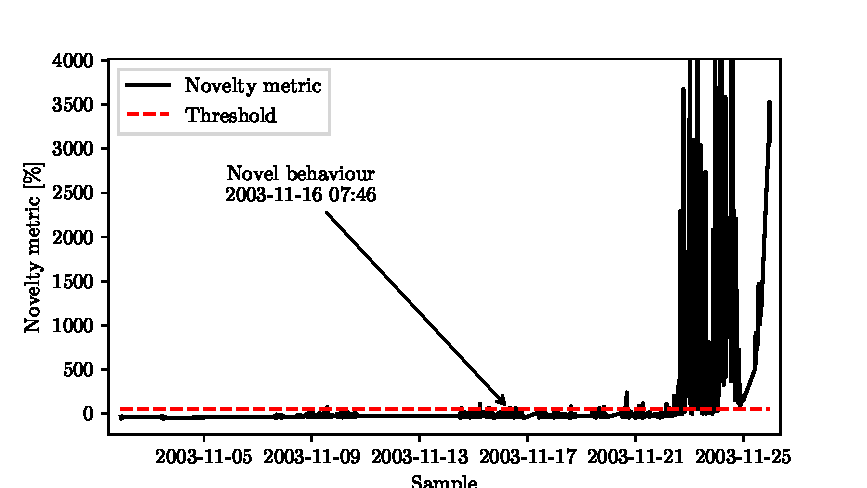
\includegraphics{images/IMS/Novelty_01_500samples_bearing3x.pdf}
    \caption{Results of \gls{nd} for the test $\text{n}^\circ$1 of \gls{ims} dataset (K-means)}
    \label{fig:NoveltyScore_01} 
\end{figure}

\begin{figure}
    \centering
    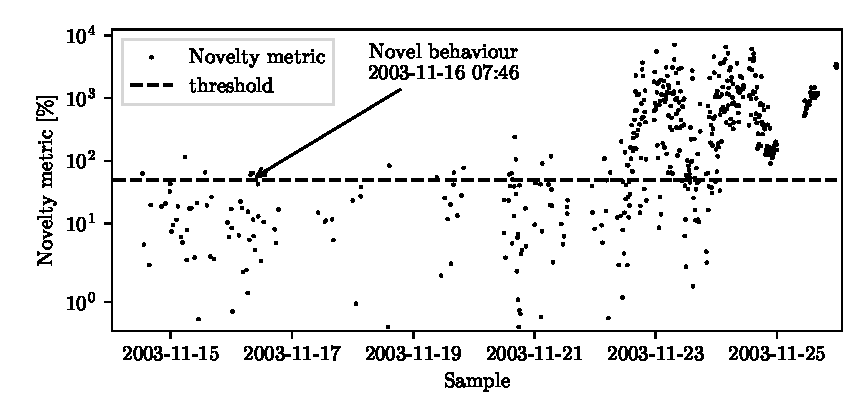
\includegraphics{images/IMS/Novelty_01_500samples_bearing3x_detail.pdf}
    \caption{Results of \gls{nd} for the test $\text{n}^\circ$1 of \gls{ims} dataset (K-means) - detailed view}
    \label{fig:NoveltyScore_01_detail} 
\end{figure}

\subsection{Training - \gls{dbscan}}
Using the same partition of the dataset as for the K-means training, we can train a \gls{dbscan} model. In this case, the silhouette score has to be used to select a suitable value of the radius $\varepsilon$. As shown in \autoref{fig:silscore_dbscan}, the optimal value is 8, which corresponds correctly to the generation of two \gls{glo:clust}s.

\begin{figure}
    \centering
    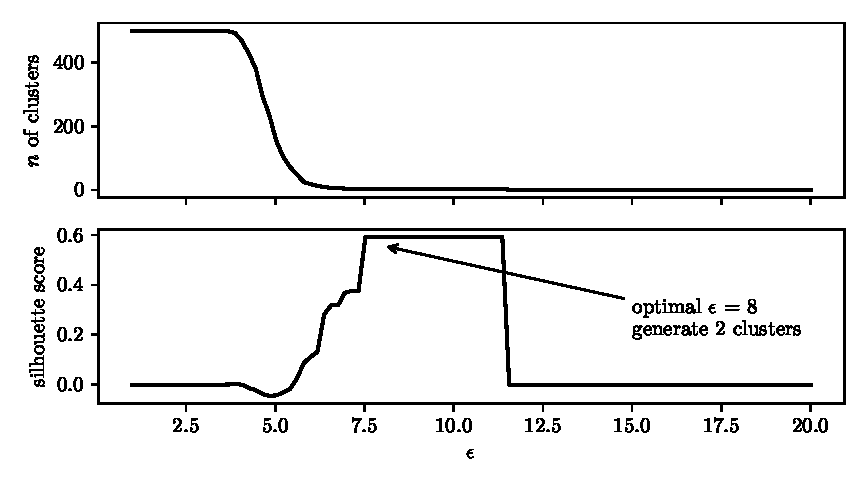
\includegraphics{images/IMS/InertiaScore_01_dbscan.pdf}
    \caption{Silhouette score for \gls{glo:clust}ing the test $\text{n}^\circ$1 of \gls{ims} dataset (\gls{dbscan})}
    \label{fig:silscore_dbscan}
\end{figure}

\subsection{\gls{nd} Validation - \gls{dbscan}}
As it has been done for the K-means, the validation partition of the dataset is now used for performing \gls{nd} with the \gls{dbscan} model, as described in \autoref{sec:dbscan_eval}. The result is shown in \autoref{fig:NoveltyScore_01_dbscan}, where we can see that the \gls{dbscan} model detects the novelty at 2003-11-22 15:06, that is quite early, but not as early as the K-means model. This is because the metric generated by the \gls{dbscan} model has a greater variance so, instead of increasing consistently, it overshoots the threshold quite before this time but fails to consistently stay above the threshold. 

\begin{figure}
    \centering
    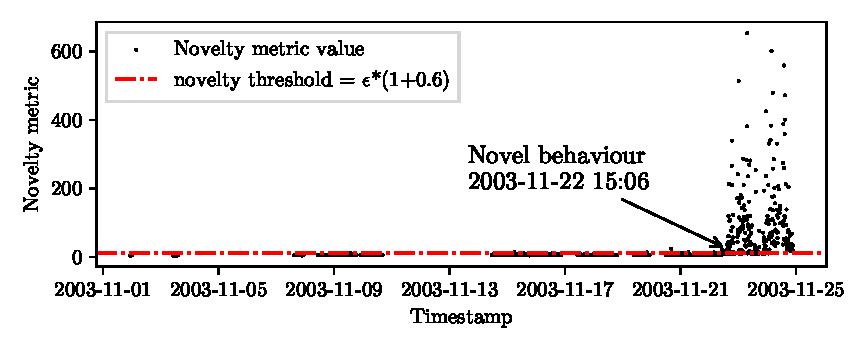
\includegraphics{images/IMS/Novelty_01_500samples_bearing3x_dbscan.pdf}
    \caption{Results of \gls{nd} for the test $\text{n}^\circ$1 of \gls{ims} dataset (\gls{dbscan})}
    \label{fig:NoveltyScore_01_dbscan}
\end{figure}

\subsection{Training - \gls{gmm}}
Let's now try with the \gls{gmm} model. The metric for selecting the number of \gls{glo:clust}s is now the \gls{bic} and the \gls{aic}, as shown in \autoref{fig:bic_aic_gmm}. The two metrics diverge but, as discussed in \autoref{sec:gauss_train}, the \gls{aic} tends to perform better. In this case, minimizing the \gls{aic} leads to select 25 as the number of \gls{glo:clust}s, which is much more than what was selected with the K-means, but still a reasonable choice, also considering that the \gls{gmm} is a soft \gls{glo:clust}ing algorithm and that we are using the density as a metric to perform \gls{nd}.

\begin{figure}
    \centering
    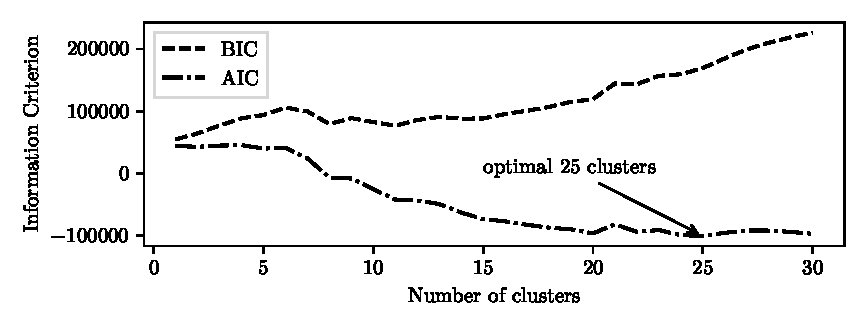
\includegraphics{images/IMS/BICAIC_GMM.pdf}
    \caption{\gls{bic} and \gls{aic} for \gls{glo:clust}ing the test $\text{n}^\circ$1 of \gls{ims} dataset (\gls{gmm})}
    \label{fig:bic_aic_gmm}
\end{figure}

\subsection{\gls{nd} Validation - \gls{gmm}}
The validation partition of the dataset is now used for performing \gls{nd} with the \gls{gmm} model. The result is shown in \autoref{fig:NoveltyScore_01_gmm}, where we can see that the \gls{gmm} model detects the novelty at 2003-11-22 03:47. The considerations about this result are the same as for the \gls{dbscan} model, and in fact, the timestamp of the detection event is really close to the one obtained with \gls{dbscan}. In \autoref{fig:NoveltyScore_01_gmm}, the metric (density value) appears in coloured dots, as each colour represents the \gls{glo:clust} to which the \gls{glo:snap} has been assigned.
\begin{figure}
    \centering
    \includegraphics{images/IMS/Novelty_01_500samples_bearing3x_gmm.pdf}
    \caption{Results of \gls{nd} for the test $\text{n}^\circ$1 of \gls{ims} dataset (\gls{gmm})}
    \label{fig:NoveltyScore_01_gmm}
\end{figure}

\subsection{\gls{nd} Validation - Bayesian \gls{gmm}}
The other Gaussian model is the \gls{bgmm}, since this approach is totally unsupervised, only the validation results are reported here. The result is shown in \autoref{fig:NoveltyScore_01_bgmm}, where we can see that the \gls{bgmm} model detects the novelty around the same time as the \gls{gmm} model, at 2003-11-22 03:45.

In both \gls{gmm} and \gls{bgmm} the metric (density value) spans a lot of decades, so the plots are done on a logarithmic scale.

\begin{figure}
    \centering
    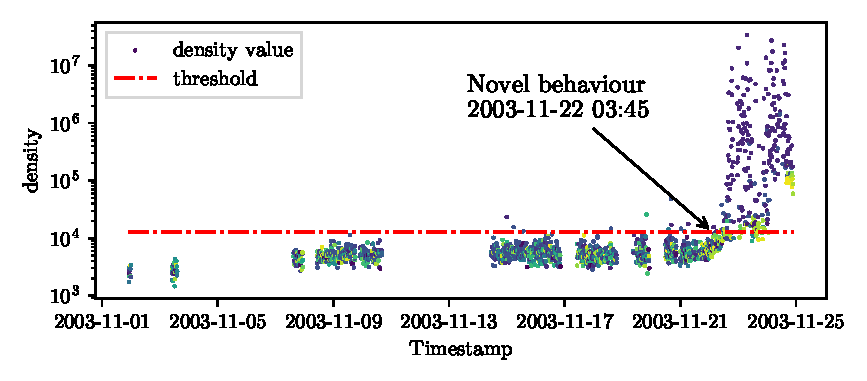
\includegraphics{images/IMS/Novelty_01_500samples_bearing3x_GMM_bayesan.pdf}
    \caption{Results of \gls{nd} for the test $\text{n}^\circ$1 of \gls{ims} dataset (\gls{bgmm})}
    \label{fig:NoveltyScore_01_bgmm}
\end{figure}

\subsection{\gls{nd} Validation - \gls{nu_svm}}
The next algorithm to test is the \gls{nu_svm}. Again, this is totally unsupervised, so only the validation results are reported here. The novelty metric evolution over time is shown in \autoref{fig:NoveltyScore_01_nusvm}, where we can see that the \gls{nu_svm} model detects the novelty at 2003-11-22 14:56, which is comparable with the \gls{dbscan} and \gls{gmm} models.

\begin{figure}
    \centering
    \includegraphics{images/IMS/Novelty_01_500samples_bearing3x_nusvm.pdf}
    \caption{Results of \gls{nd} for the test $\text{n}^\circ$1 of \gls{ims} dataset (\gls{nu_svm})}
    \label{fig:NoveltyScore_01_nusvm}
\end{figure}

\subsection{\gls{nd} Validation - \gls{iforest}}
The second last technique to test is the one based on the \gls{iforest} model. The result is shown in \autoref{fig:NoveltyScore_01_iforest}, where we can see that the \gls{iforest} model detects the novelty at 2003-11-16 10:08:46, which is a good result comparable with the K-means model. The problem with the metric of the \gls{iforest} is that it increases a lot the variance around the \gls{nd} event, but the mean does not increase consistently, so a lot of \gls{glo:snap}s are discarded as outliers, before the \gls{nd} event. 

This is, in my opinion, a promising approach. With these settings a lot of \gls{glo:snap}s are discarded as outliers, but with a different outlier filter, based on the percentage of novelty samples in a window, the \gls{iforest} model could perform even better.
\begin{figure}
    \centering
    \includegraphics{images/IMS/Novelty_01_500samples_bearing3x_iforest.pdf}
    \caption{Results of \gls{nd} for the test $\text{n}^\circ$1 of \gls{ims} dataset (\gls{iforest})}
    \label{fig:NoveltyScore_01_iforest}
\end{figure}

\subsection{\gls{nd} Validation - \gls{lof}}
The last algorithm to test is the \gls{lof}. The result is shown in \autoref{fig:NoveltyScore_01_lof}, where we can see that the \gls{lof} model detects the novelty at 2003-11-16 07:49, which is a good result comparable with the K-means model. It doesn't have the same problem as the \gls{iforest}, as there aren't as many discarded \gls{glo:snap}s before the \gls{nd} event.

\begin{figure}
    \centering
    \includegraphics{images/IMS/Novelty_01_500samples_bearing3x_lof.pdf}
    \caption{Results of \gls{nd} for the test $\text{n}^\circ$1 of \gls{ims} dataset (\gls{lof})}
    \label{fig:NoveltyScore_01_lof}
\end{figure}

\subsection{Comparison of the results}

\subsubsection{Comparison between the models}

\begin{table}
    \centering
    \caption{Comparison of the results for the test $\text{n}^\circ$1 of \gls{ims} dataset.}
    \label{tab:ims01_comparision}
    \begin{tabular}{lrr} 
    \toprule
    \textbf{Algorithm} & \textbf{\gls{nd} event} & \textbf{\gls{glo:leadtime} }{[}min] \\ 
    \hline
    K-means & 2003-11-16 07:46 & \textbf{13913} \\
    \gls{dbscan} & 2003-11-22 15:06 & 4833 \\
    \gls{gmm} & 2003-11-22 03:47 & 5513 \\
    \gls{bgmm} & 2003-11-22 03:45 & 5514 \\
    \gls{nu_svm} & 2003-11-22 14:56 & 4844 \\
    \gls{iforest} & 2003-11-16 10:08 & 13771 \\
    \gls{lof} & 2003-11-16 07:48 & 13912 \\
    {P2P} without any \gls{ml} & 2003-11-22 16:06 & 4774 \\
    \bottomrule
    \end{tabular}
\end{table}

In \autoref{tab:ims01_comparision}, the results of all the previous tests are resumed, together with the result of performing \gls{nd} without any machine learning algorithm, but just setting a threshold on the P2P value of the time-series, as it was previously shown in \autoref{fig:IMS_TD_features}. This last basic approach detects the novelty around the afternoon of 2003-11-22. 

The \gls{nu_svm} and the \gls{dbscan} models are not performing much better than not even using machine learning (at least on this dataset signal). The \gls{gmm} and \gls{bgmm} models are performing slightly better, but the margin is so low that the result may be biased by the threshold setting. The \gls{iforest}, \gls{lof} and K-means models are performing better, they are all very close to detecting the novelty, around 14000 min = 9.7 days before the end of the test. The K-means model is the one performing the best, but just slightly better than the \gls{iforest} and \gls{lof} models so, again, this small difference may not be significant. However, as discussed in the previous chapters, the K-means model will be used in the rest of the work, as it is also the most simple and interpretable model.


\subsubsection{Comparison with another approach}
As anticipated in the \autoref{ch:state_of_the_art}, about the State of the Art, the signal of the same bearing (Bearing 3x) of this same test has been used in \cite{Umberto}. In their research, the authors used a different approach, based on regression, and obtained the result reported in \autoref{fig:umbertoresult}


\subsubsection{Comment about the comparison}
Every system that outputs a warning based on a trigger on a threshold is highly sensitive to the value of the threshold itself. This means that the comparison of the results is not straightforward, and quite opinable, because selecting a low threshold will make almost every system trigger earlier. The measure to take into consideration, in my opinion, is how many false positives are generated if the threshold is lowered, and how small the variance of the metric is. A high variance, on this dataset, means that the system is very sensitive while evaluating quite similar signals.

\subsection{\gls{rul} Predictions validation - K-means}
After the \gls{nd} event, the \gls{mla} starts predicting the future evolution of the novelty metric, and it superimposes the prediction curve to the same plot displayed to the user. The fitting procedure is the closed form solution of the \gls{ls} problem applied to an exponential curve of \autoref{eq:exp_degradation_2}, as described in \autoref{sec:predictions}. The samples used for the regression of the curve are the last 230 before the current one. This parameter of the \gls{glo:frmwrk} is configurable in the \texttt{.yaml} file. 

Some good predictions are shown in \autoref{fig:RULPredictions01}. The \gls{rul} is the difference between the intercept of the prediction curve and another threshold, higher than the one used for \gls{nd}, and the current time. In the figure, the blue line is a prediction made just a few hours after the \gls{nd} event (the vertical dashed line marks the time of the prediction). The same concept applies to the other predictions performed in later times.

In some circumstances, the novelty metric starts decreasing slightly, on average, as can be seen around 2003-11-21. In this case, if the novelty metric has this behaviour for several \gls{glo:snap}s ($\approx 230$), the fitted curve will be a decreasing exponential, as shown in \autoref{fig:RULPredictions01_fail}. 

If this situation occurs, the intercept with the threshold does not exist, and the \gls{rul} prediction fails, so the interpretation of the \gls{rul} is left to the user. In some cases, the defect in a system can \quoted{self-heal} (for example a crack in a bearing can be polished with the use \cite{IMSpaper}). If this behaviour is possible for the system, this situation can be interpreted as a sign that the system is going to return to normality. Otherwise, the user can retain the previous \gls{rul} prediction as the \gls{rul} of the system.

\begin{figure}
    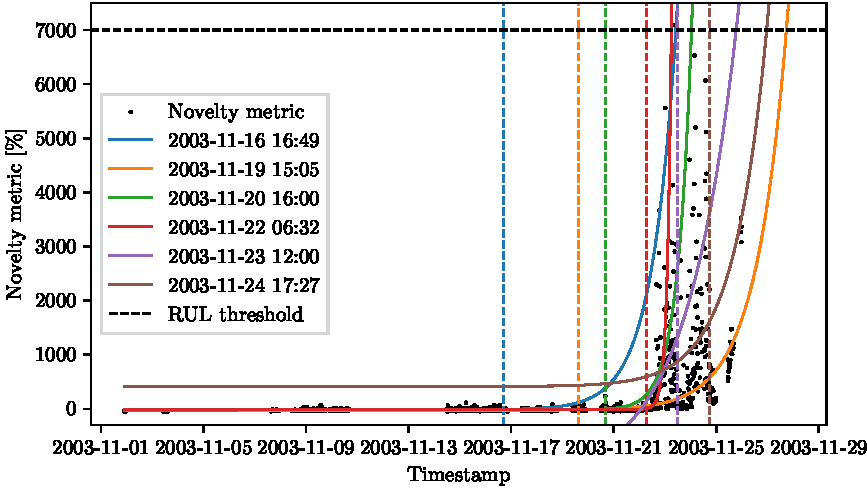
\includegraphics{images/IMS/Novelty_01_500samples_bearing3x_predictions.pdf}
    \caption{\gls{rul} prediction at different instants after the \gls{nd} event (dashed lines are the instants of the predictions corresponding to the same-colour solid line prediction)}
    \label{fig:RULPredictions01}
\end{figure}

\begin{figure}
    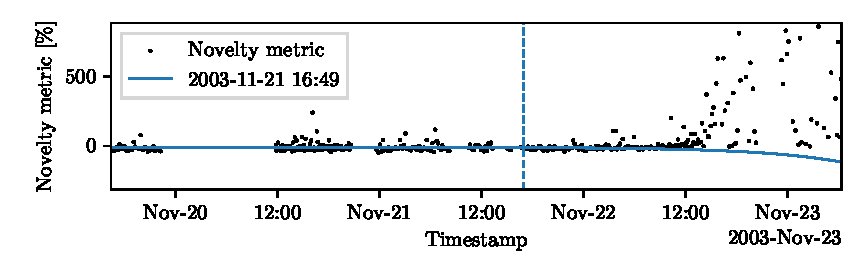
\includegraphics{images/IMS/Novelty_01_500samples_bearing3x_predictions_failed.pdf}
    \caption{Failed \gls{rul} prediction.}
    \label{fig:RULPredictions01_fail}
\end{figure}

\subsection{Retraining,  evaluating and predicting after \gls{nd} event}
If the user, after the \gls{nd} event, performs an investigation that leads to the belief that the system is still healthy, the user can turn the \gls{mla} in \emph{retrain} mode. In this case, the \gls{glo:snap}s that are in the quarantine collection, are moved to the healthy collection (faulty if the instance is for \gls{fd} and the investigation reveals that the fault is real). 
The model is then retrained with the new data with the same procedure used for the first training (silhouette and inertia scores are computed and the user is asked to confirm the number of \gls{glo:clust}s).

Let's investigate what would have happened if the user declared the system healthy at 2003-11-23 00:00, in the previous scenario of  \quoted{Bearing 3 x} signal in the \gls{ims} dataset. The \gls{mla} suggests that the best number of \gls{glo:clust}s is still two, so it has been retrained with the new data. The result of the updated model performing \gls{nd} is shown in \autoref{fig:NoveltyScore_01_retrained}. The predictions of the \gls{rul} are shown in \autoref{fig:RULPredictions01_retrained}. 

This test shows that in an increasingly decaying system retrained with data very close to the fault condition the \gls{mla} is able to detect the fault again. This comes at the cost of a later detection, and the first predictions after the \gls{nd} event are not as good as the previous ones. Anyway, the \gls{rul} predictions still become more accurate as time passes, and the \gls{rul} prediction at the end of the test is still quite accurate (on the same day of the event). 

Another consideration is about the \gls{rul} threshold: since the model has been retrained with \quoted{worse} data, the threshold for the \gls{rul} prediction should be set to a lower value, because now the \gls{glo:clust}s are either more in quantity, distorted or bigger, so it is unlikely that the novelty metric can still reach the same high values estimated before the retraining.

An intuition about why the sensitivity of the system is reduced after the retraining comes by examining the scatter plot of the \gls{glo:snap}s in the \gls{glo:feature} space, shown in \autoref{fig:Clusters_novelty}, where all the \gls{glo:snap}s extracted from the dataset are displayed. The \gls{glo:clust}s are more elongated and much bigger. These shapes arise gradually from the original ones of \autoref{fig:Clusters} so, by performing a retrain, both the effect of producing bigger \gls{glo:clust}s and one of the \gls{glo:clust}s being much more elongated play a role in reducing the sensitivity of the \gls{mla}.

\begin{figure}
    \centering
    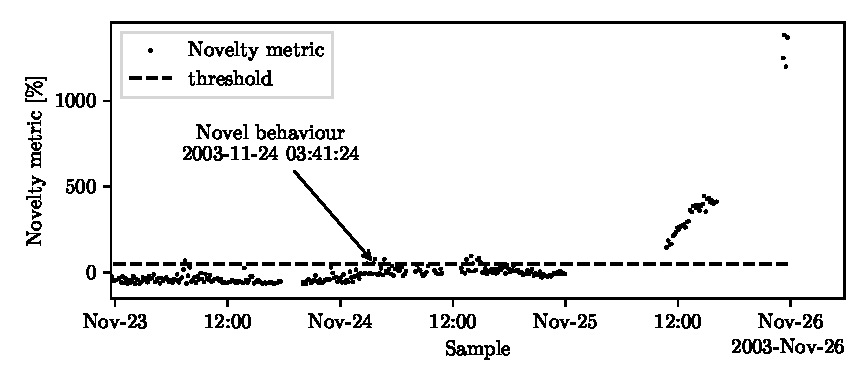
\includegraphics{images/IMS/Novelty_01_500samples_bearing3x_retrained.pdf}
    \caption{Results of \gls{nd} for the test $\text{n}^\circ$1 of \gls{ims} dataset (K-means) - retrained model}
    \label{fig:NoveltyScore_01_retrained}
\end{figure}

\begin{figure}
    \centering
    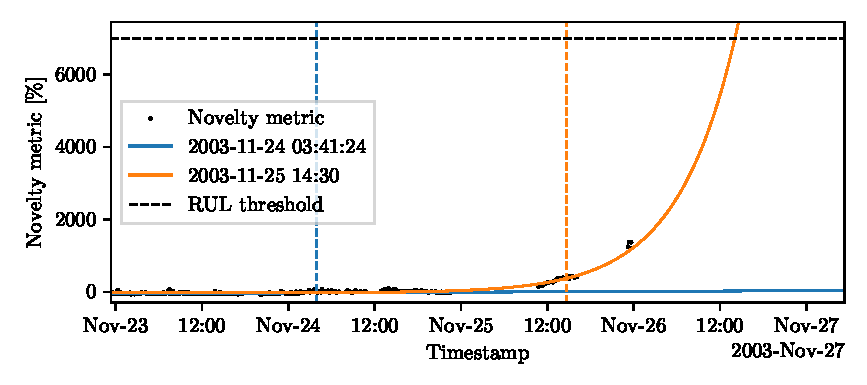
\includegraphics{images/IMS/Novelty_01_500samples_bearing3x_predictions_retrained.pdf}
    \caption{\gls{rul} prediction at different instants after the \gls{nd} event with the retrained model (dashed lines are the instants of the predictions corresponding to the same-colour solid line prediction)}
    \label{fig:RULPredictions01_retrained}
\end{figure}

\begin{figure}
    \centering
    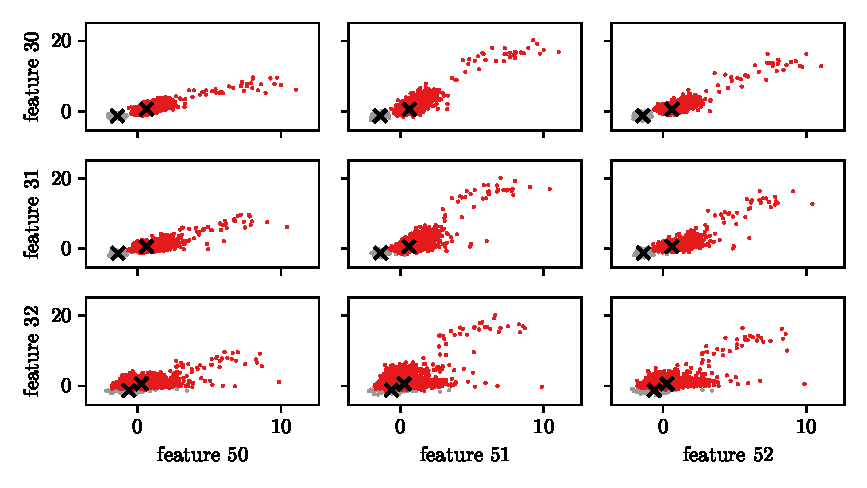
\includegraphics{images/IMS/Clusters_novelty.pdf}
    \caption{Scatterplot of all the $\gls{glo:snap}$ for the test $\text{n}^\circ$1 of \gls{ims} dataset}
    \label{fig:Clusters_novelty}
\end{figure}

